\subsection{Vectors}

\begin{description}
  \item[$a$] Scalar quantity.
  \item[$\bvec{a}$] Vector in n-dimensional space. $\norm{\bvec{a}} = a$.
  \item[$\bhat{a}$] Unit vector in n-dimensional space. $\bhat{a} = \bvec{a}/a$ and $\norm{\bhat{a}} = 1$.
\end{description}

\subsection{Angles}

Since many of the theorems in this paper involve polar coordinates, we define two different types of angle measurements: the standard measurement, and a directional measurement. All angles are measured in radians.

In the standard measurement, angles are in $[0, 2\pi]$ and are measured counterclockwise. In the directional measurement, angles are in $[-\pi, \pi]$ and the measurement direction is indicated by an arrow on the figure.

\begin{figure}[H]
  \centering
  \begin{subfigure}[b]{0.4\textwidth}
    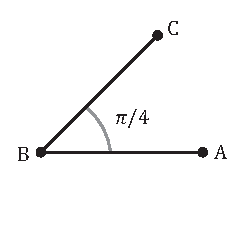
\includegraphics[width=\textwidth]{angle_def_1.eps}
    \caption{}
    \label{fig:angle-def-1}
  \end{subfigure}
  \qquad \qquad
  \begin{subfigure}[b]{0.4\textwidth}
    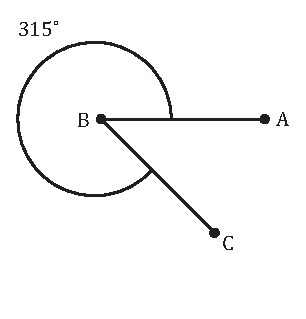
\includegraphics[width=\textwidth]{angle_def_2.eps}
    \caption{}
    \label{fig:angle-def-2}
  \end{subfigure}
  \caption{Standard angle notation (no arrow)}
\end{figure}

\begin{figure}[H]
  \begin{subfigure}[b]{0.4\textwidth}
    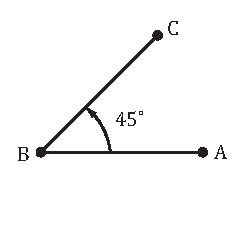
\includegraphics[width=\textwidth]{angle_def_3.eps}
    \caption{}
    \label{fig:angle-def-3}
  \end{subfigure}
  \qquad \qquad
  \begin{subfigure}[b]{0.4\textwidth}
    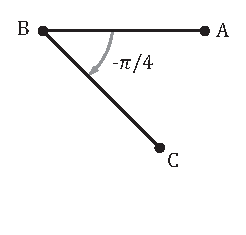
\includegraphics[width=\textwidth]{angle_def_4.eps}
    \caption{}
    \label{fig:angle-def-4}
  \end{subfigure}
  \caption{Directional angle notation (arrow)}
\end{figure}